\documentclass{article}
\usepackage{listings}
\usepackage{color}
\usepackage{hyperref}
\usepackage{amsmath}
\usepackage{graphicx}

\definecolor{gray}{rgb}{0.5,0.5,0.5}
\lstset{
  basicstyle=\ttfamily\small,
  commentstyle=\color{gray},
  breaklines=true,
  frame=single,
  language=bash,
  showstringspaces=false
}

\title{Understanding GitHub Workflows, Tags, Releases, and Build Artifacts}
\author{}
\date{}

\begin{document}
\maketitle

\section{What is a Workflow?}
A \textbf{workflow} in GitHub Actions is an automated process defined in a YAML file within the \texttt{.github/workflows} directory of a repository. It consists of one or more jobs and steps, which can include shell scripts or GitHub-provided actions.

\begin{figure}[h]
  \centering
  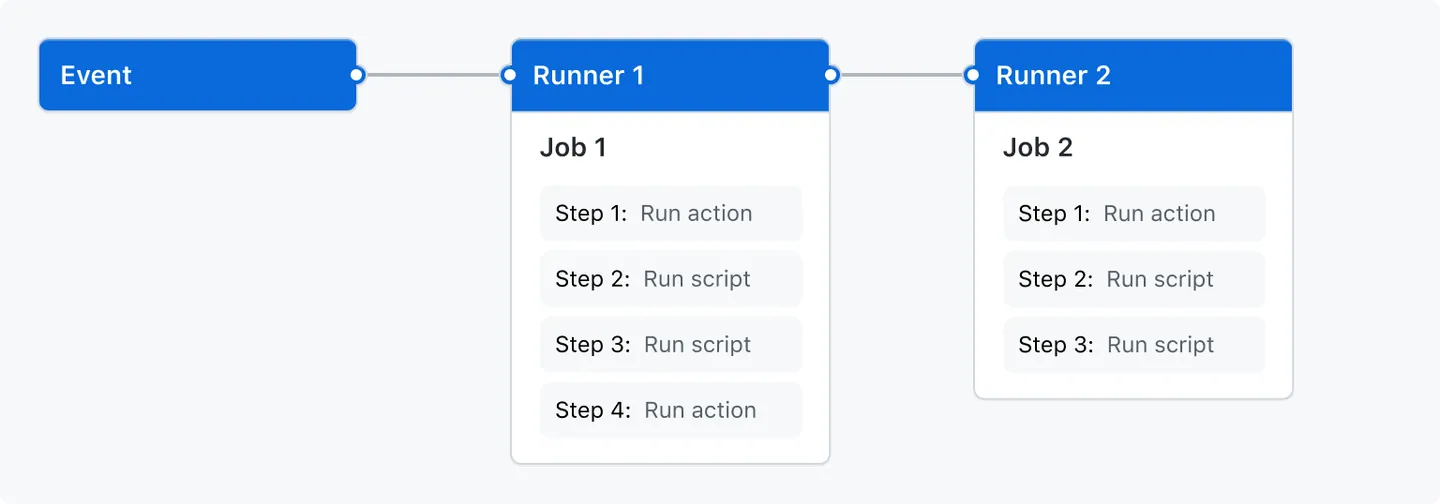
\includegraphics[width=0.7\textwidth]{1.png}
  \caption{Relationships.}
\end{figure}

Workflows are run in GitHub-hosted virtual machines (called \textbf{runners}). These are temporary, isolated environments that execute your code automatically when triggered (e.g., by pushing code, opening a pull request, or creating a release). Workflows are defined in the .github/workflows directory in a repository. A repository can have multiple workflows

The operations inside a workflow (like running tests, building software, or uploading files) are similar to what a developer could do on their own machine, but automated and standardized across environments.

\section{Example Workflow Explained Line-by-Line}
Below is a sample workflow and a line-by-line explanation using inline comments:

\begin{lstlisting}[language=bash]
# Name of the GitHub Actions workflow
name: Compile LaTeX document and Release

# This section defines when the workflow should be triggered
on:
  push:
    tags:
      - '*'  # Trigger the workflow on any Git tag push

# Define the jobs that will run in this workflow
jobs:
  build-and-release:  # Name of the job
    runs-on: ubuntu-latest  # Use the latest Ubuntu runner for this job

    steps:
    # Step 1: Check out the repository code into the runner
    - uses: actions/checkout@v2
      with:
        submodules: 'recursive'  # Also initialize and update any Git submodules

    # Step 2: Set up environment variables for the filenames
    - name: Prepare Filename
      run: |
        REPO_NAME="${GITHUB_REPOSITORY##*/}"  # Extract the repo name (e.g., "myrepo" from "user/myrepo")
        echo "REPO_TEX_NAME=${REPO_NAME}.tex" >> $GITHUB_ENV  # Save LaTeX filename as env variable
        echo "REPO_PDF_NAME=${REPO_NAME}.pdf" >> $GITHUB_ENV  # Save output PDF filename as env variable

    # Step 3: Rename the default LaTeX file (worksheet.tex) to match the repo name
    - name: Rename worksheet.tex
      run: mv worksheet.tex ${{ env.REPO_TEX_NAME }}  # Rename worksheet.tex to match the expected LaTeX filename

    # Step 4: Compile the LaTeX file into a PDF using a LaTeX GitHub Action
    - name: Compile LaTeX Document
      uses: xu-cheng/latex-action@v2  # Use a prebuilt LaTeX compiler action
      with:
        root_file: ${{ env.REPO_TEX_NAME }}  # Specify the LaTeX file to compile

    # Step 5: Create a GitHub Release for the current tag
    - name: Create Release
      id: create_release  # Set an ID so we can refer to this step's outputs later
      uses: actions/create-release@v1
      env:
        GITHUB_TOKEN: ${{ secrets.GITHUB_TOKEN }}  # GitHub provides this token to authenticate API requests
      with:
        tag_name: ${{ github.ref }}  # Use the current tag (e.g., refs/tags/v1.0)
        release_name: Release ${{ github.ref }}  # Name of the release
        draft: false  # Publish the release immediately
        prerelease: false  # Mark it as a stable release

    # Step 6: Upload the compiled PDF as an asset to the release
    - name: Upload PDF as Release Asset
      uses: actions/upload-release-asset@v1
      env:
        GITHUB_TOKEN: ${{ secrets.GITHUB_TOKEN }}  # Authenticate upload
      with:
        upload_url: ${{ steps.create_release.outputs.upload_url }}  # Use the upload URL from the previous step
        asset_path: ./${{ env.REPO_PDF_NAME }}  # Path to the compiled PDF file
        asset_name: ${{ env.REPO_PDF_NAME }}  # Name of the asset on the release page
        asset_content_type: application/pdf  # Specify MIME type
\end{lstlisting}

\section{What is a Git Tag?}
A \textbf{Git tag} is a pointer to a specific commit in a Git repository. It is often used to mark specific versions (e.g., \texttt{v1.0.0}) in the project's history.

Tags can be created using:
\begin{lstlisting}
git tag v1.0.0
git push origin v1.0.0
\end{lstlisting}

\subsection*{Tags on GitHub}
On GitHub, tags appear under the \texttt{Tags} tab in the "Releases" section of the repository. Tags themselves are lightweight and contain no additional metadata beyond the commit they reference.

\section{Tags vs Releases}
A \textbf{release} on GitHub is a more formal version of a tag. When you create a release, you can attach:
\begin{itemize}
    \item Release notes (markdown description)
    \item Binary files or build artifacts
    \item Version information
\end{itemize}

You can create a release from a tag either manually on GitHub or automatically through a workflow.

\section{What is a Build Artifact?}
A \textbf{build artifact} is a file or group of files produced as a result of a build process — e.g., compiled binaries, package archives, or test reports.

In GitHub Actions:
\begin{itemize}
    \item Artifacts are uploaded during a job using \texttt{actions/upload-artifact}.
    \item They are stored temporarily in GitHub's storage (usually for 90 days).
    \item They can be downloaded manually from the Actions tab.
\end{itemize}

\section{Creating a Release from an Artifact}
When a release is created, it can include build artifacts by either:
\begin{itemize}
    \item Downloading them from previous jobs and attaching them to the release manually.
    \item Using GitHub Actions like \texttt{softprops/action-gh-release} to automatically publish artifacts stored during the workflow.
\end{itemize}

This allows users to download executable files or packages directly from the release page, making it easier to distribute software.

\end{document}
